\documentclass[12pt]{article}
\usepackage{geometry}
\geometry{a4paper, margin=1in}
\usepackage{booktabs}
\usepackage{tabularx}
\usepackage{float}
\usepackage{graphicx}
\usepackage{enumitem}
\usepackage{amsmath}
\usepackage{array}
\usepackage{hyperref}
\hypersetup{colorlinks=true, linkcolor=blue, citecolor=blue, urlcolor=blue}

\newcolumntype{L}[1]{>{\raggedright\arraybackslash}p{#1}}

\title{Evaluating Verifiability in the Privacy Preserving Data Analytics Engine (E-Privacy)}
\author{Dilmith D. L. S., Hansana O. G. V., Vidyananda H. K. H.}
\date{September 25, 2026}

\begin{document}
\maketitle

\section{Introduction}
In E-Privacy, a Data Owner (e.g.\ a bank) encrypts its records locally with Paillier (2048-bit modulus), uploads only ciphertext to the cloud, and asks the cloud's Homomorphic Compute Engine to return aggregates such as the sum and average of \texttt{Transaction\_Amount} over its 2,000,000 transaction records. Confidentiality is guaranteed because the cloud never holds the private key. \emph{Correctness}, however, is not: an untrusted cloud could silently drop records, include stale ones, or return a wrong ciphertext, and the Data Owner would decrypt a plausible-looking but wrong number.

The Swiss e-voting system faces the same problem with ballots and tallies, and answers it with two properties, which this report applies to E-Privacy:
\begin{itemize}[leftmargin=1.5em]
    \item \textbf{Individual verifiability} -- the Data Owner can check that \emph{its own} uploaded records were stored as uploaded and were actually used in the query it asked for.
    \item \textbf{Universal verifiability} -- \emph{any} third party (e.g.\ a financial regulator or external auditor) can check that the published result was correctly computed from the committed ciphertexts and correctly decrypted, without the private key and without seeing any individual record.
\end{itemize}

\subsection{Design Basis}
\begin{itemize}[leftmargin=1.5em]
    \item[V1.] As in the SRS (A2, A3), there is one trusted Data Owner per deployment holding the Paillier private key, and the cloud is honest-but-curious; verifiability is the mechanism that turns any deviation by the cloud into a \emph{detectable} event.
    \item[V2.] The Verifiable Computation \& Audit Module (FR-6) is extended into an append-only, hash-chained \textbf{bulletin board}, readable by the Data Owner and by auditors authorised through the Access Control \& Policy Engine (FR-4).
    \item[V3.] Each board entry is hashed with SHA-256 and signed by the cloud with ECDSA-P256, so the cloud cannot later deny or rewrite what it published.
    \item[V4.] Only aggregates over at least a policy-defined minimum number of records are published (FR-4), so revealing an aggregate result does not reveal an individual value.
\end{itemize}

\section{Protocol}
Figure~\ref{fig:verifiability} shows how both properties fit into the existing E-Privacy query flow (upload $\rightarrow$ API Gateway $\rightarrow$ Homomorphic Compute Engine $\rightarrow$ Audit Log $\rightarrow$ local decryption).

\begin{figure}[H]
    \centering
    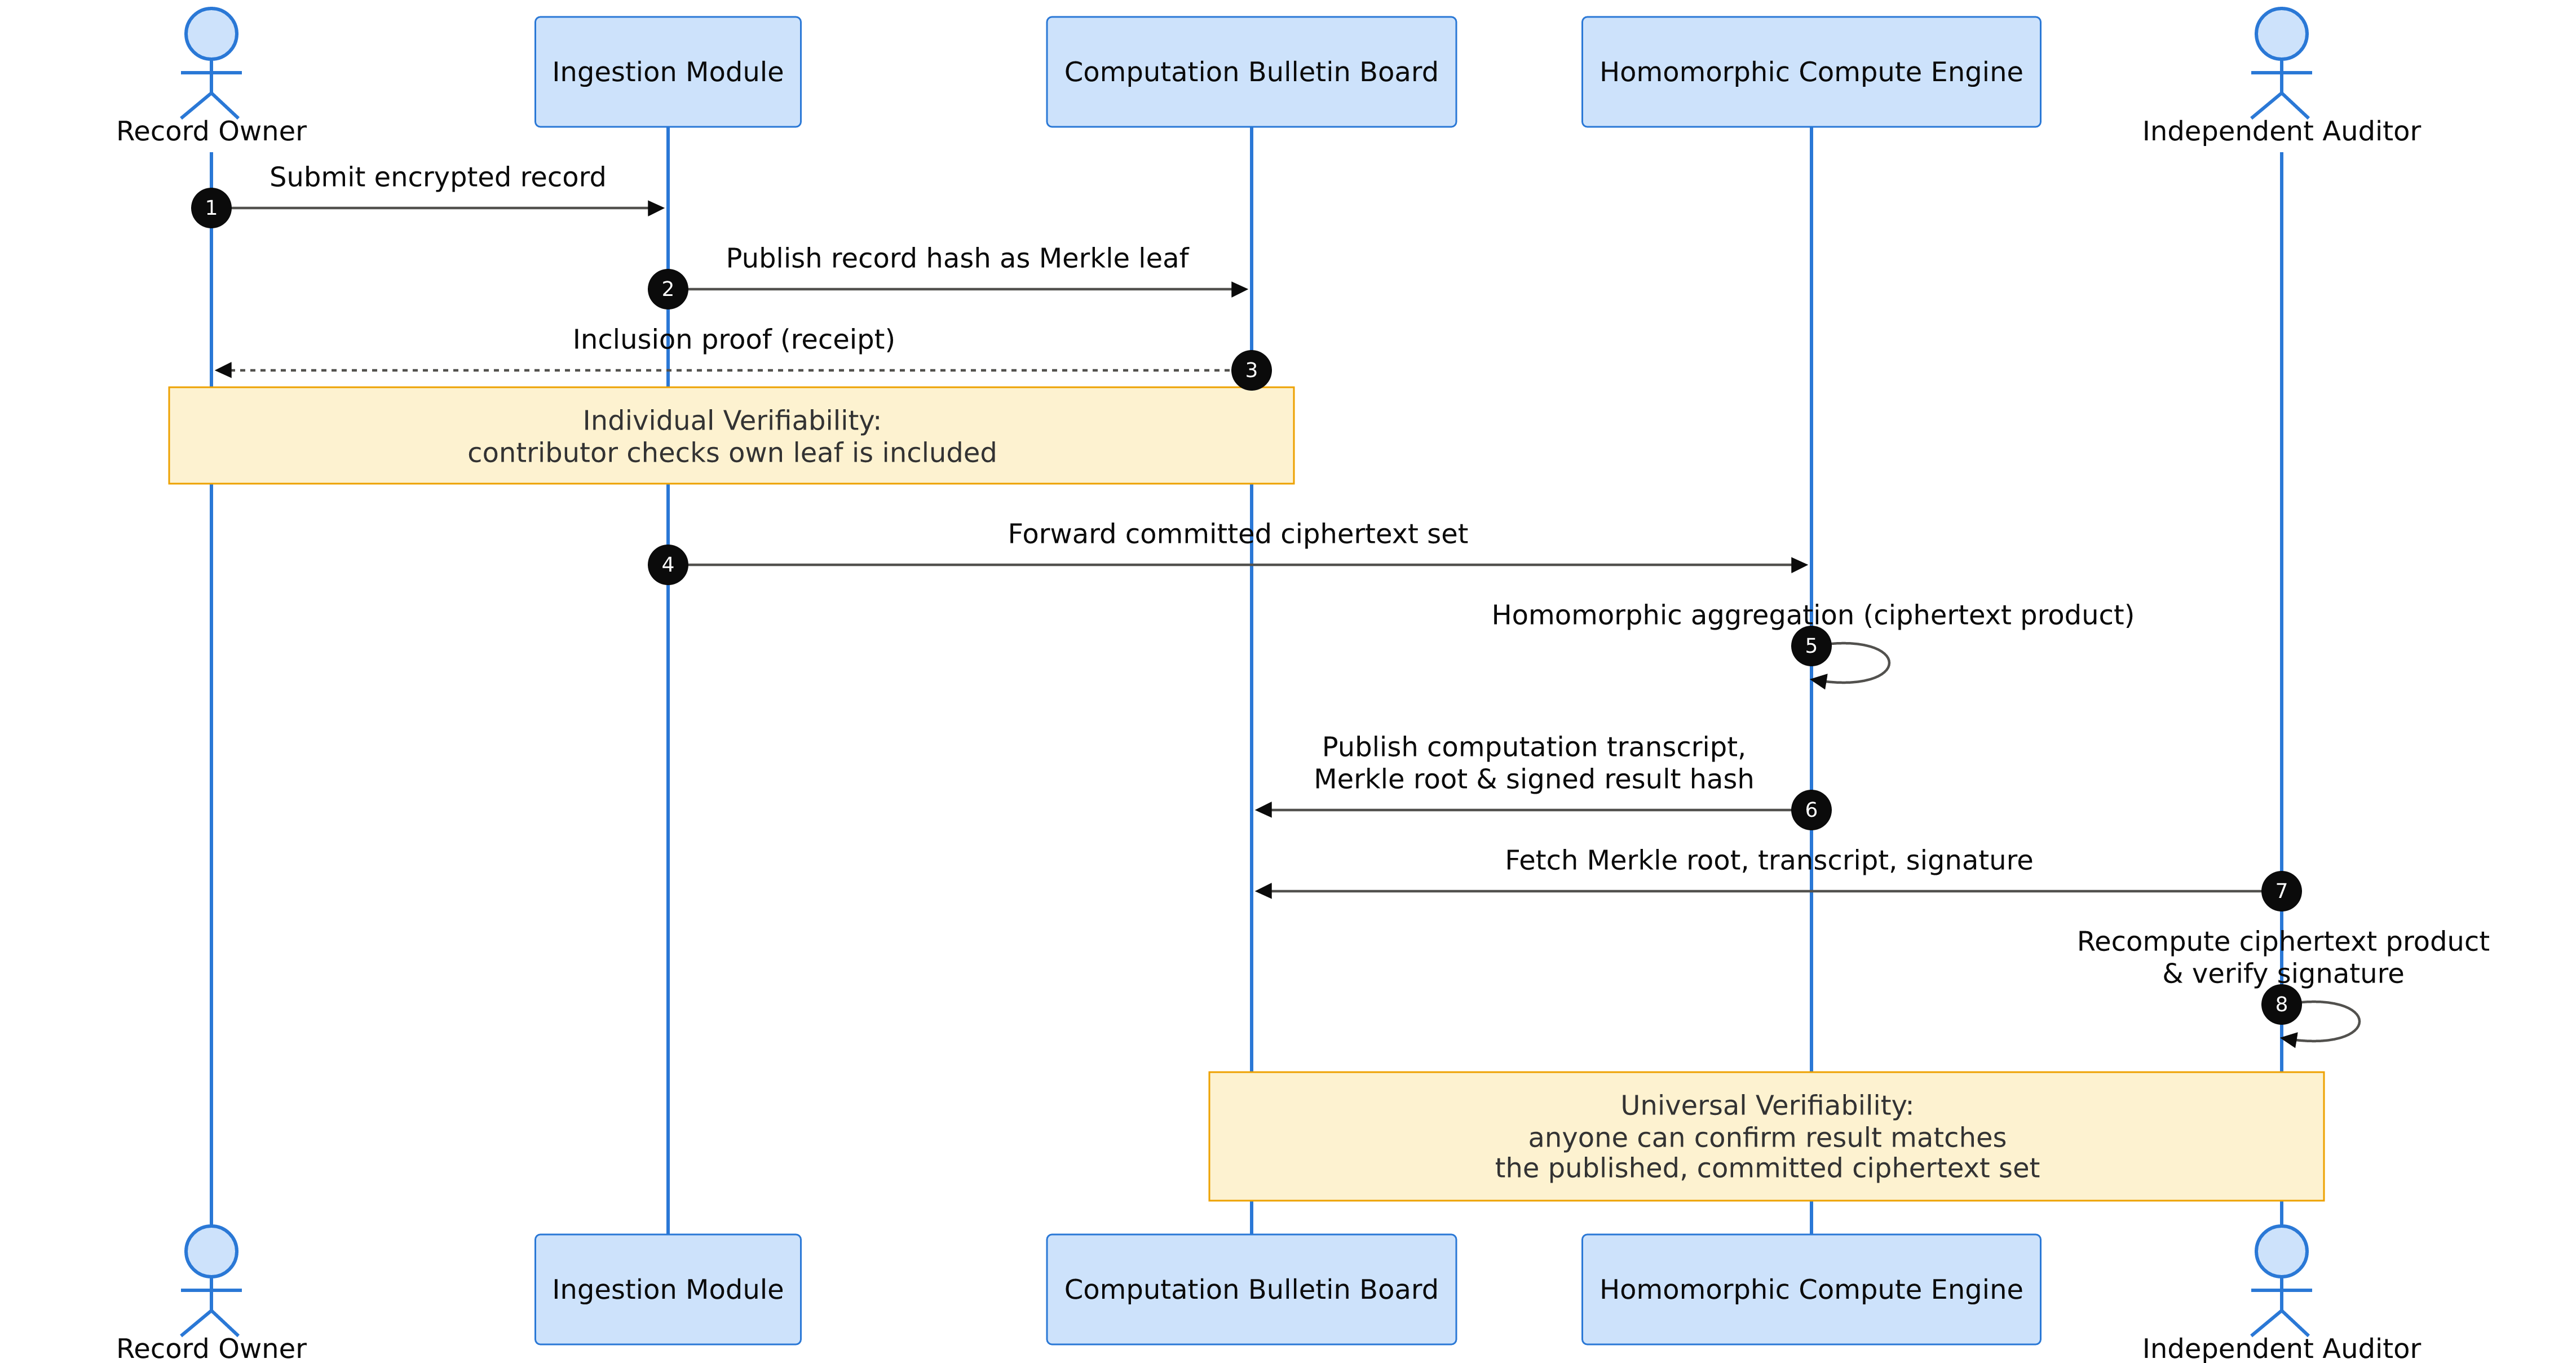
\includegraphics[width=0.95\textwidth]{sources/verifiability/verifiability-bulletin-board.png}
    \caption{Individual and universal verifiability in the E-Privacy query flow.}
    \label{fig:verifiability}
\end{figure}

\subsection{Individual Verifiability (Data Owner)}
\begin{enumerate}[leftmargin=1.5em]
    \item \textbf{Encrypted as intended.} Encryption happens only in the Data Owner's Local Encryption Client (FR-2), never in the cloud. Before upload, the client decrypts a random sample of the ciphertexts it just produced and compares them with the source rows, catching a faulty or tampered client library.
    \item \textbf{Stored as uploaded.} When the API Gateway accepts an upload batch, the SHA-256 hash of every ciphertext $c_i$ becomes a leaf of a Merkle tree on the bulletin board. The Gateway returns a signed receipt holding the new Merkle root and the inclusion proof for each leaf. The Data Owner keeps its own list of hashes and can check at any time that each record is still in the tree, unmodified.
    \item \textbf{Used in my query.} For each query, e.g.\ \texttt{SUM(Transaction\_Amount)}, the Compute Engine publishes the Merkle root and the leaf count $N$ of the exact input set it aggregated. The Data Owner checks that the root equals the one in its latest receipt and that $N = 2{,}000{,}000$. A dropped, extra or substituted record changes the root, so the result is rejected before it is trusted.
    \item \textbf{Result as computed.} The encrypted result returned by the Gateway must hash to the value the Compute Engine signed on the board; otherwise the result was swapped in transit or by the Gateway.
\end{enumerate}

\subsection{Universal Verifiability (Any Auditor)}
An auditor who holds only public information -- the Paillier public key $(n, g)$ and the bulletin board -- performs four checks:
\begin{enumerate}[leftmargin=1.5em]
    \item \textbf{Log integrity:} recompute the SHA-256 hash chain and verify every ECDSA-P256 signature, so no entry was edited or removed after publication.
    \item \textbf{Input set:} rebuild the Merkle root from the published ciphertexts and confirm it matches the root the Compute Engine signed for the query.
    \item \textbf{Computation:} recompute $C' = \prod_{i=1}^{N} c_i \bmod n^2$ and confirm $C' = C$, the signed encrypted sum. Paillier addition is deterministic on public ciphertexts, so this needs no key. The average is then $m / N$ with $N$ public, so it needs no separate proof.
    \item \textbf{Decryption:} Paillier decryption also recovers the randomness $r$ of a ciphertext. The Data Owner publishes the sum $m$ together with $r$, and the auditor checks $g^{m} \cdot r^{n} \equiv C \pmod{n^2}$. A false $m$ cannot pass this check, so even the Data Owner cannot misreport the result to a regulator.
\end{enumerate}

\section{What Verifiability Does and Does Not Guarantee}
\begin{itemize}[leftmargin=1.5em]
    \item \textbf{Detection, not prevention.} A dishonest cloud can still drop records or return a wrong ciphertext, but it cannot do so \emph{silently}. the Merkle root, the ciphertext product or a signature will not match. A cloud that refuses to publish at all causes a visible availability failure, not a hidden correctness failure.
    \item \textbf{No loss of confidentiality.} The board contains only ciphertexts, hashes, signatures and the final aggregate. Individual ciphertexts reveal nothing without the private key, and the published $r$ belongs to the aggregate ciphertext only, so it reveals nothing about any single record.
\end{itemize}

\section{Conclusion}
E-Privacy achieves individual verifiability through local encryption with spot-checks, signed Merkle inclusion receipts, and a per-query input-set root that the Data Owner compares against its own records. It achieves universal verifiability because Paillier aggregation can be recomputed by anyone from public ciphertexts, and Paillier decryption can be proven by revealing the aggregate's randomness. Together these let a Data Owner and an external auditor both confirm that a result such as the total of 2,000,000 transaction amounts is complete and correct, without trusting the cloud and without anyone other than the Data Owner seeing a single plaintext record.

\end{document}
